\section{Regulator LQR}
\subsection{Linearyzacja}
W kolejnym etapie badań podjęto się implementacji regulatora liniowo-kwadratowego. LQR jest regulatorem optymalnym (minimalizuje funkcję kosztu dla systemu zlinearyzowanego) co niezwykle zwiększa jego rangę i wartość w zastosowaniach. Jak sama nazwa wskazuje LQR stosowany jest do systemu opisanego przez liniowe równania różniczkowe (w naszym przypadku równania zlinearyzowane wokół niestabilnego punktu równowagi), a minimalizowana funkcja kosztu ma postać kwadratową. Postawiony problem można zapisać w sposób następujący:
\begin{equation}
\begin{aligned}
&0 = f(x_{0},u_{0}) \\    
&x_{0} = [0, 0, 0, 0]^T \\
&u_{0} = 0
\end{aligned}
\end{equation}
System zlinearyzowany w otoczeniu przedstawionego punktu równowagi:
\begin{equation}
\dot{x} = A\left( x-x_{0}\right)  + B\left( u-u_{0}\right)     
\end{equation}
gdzie
\begin{equation}
\label{eq:nabla}
\begin{aligned}
A = \bigtriangledown_{x}f(x_{0},u_{0})  \\
B = \bigtriangledown_{u}f(x_{0},u_{0})
\end{aligned}
\end{equation}
Różniczkując równania stanu \ref{eq:rStan} zgodnie z \ref{eq:nabla}:
\begin{equation}
\label{eq:AB}
\begin{aligned}
&\mathbf{A} =
\left( \begin{array}{cccc}
0 & 1 & 0 & 0 \\
\dfrac{mgl}{J_{sm}+ml^2} & 0 & 0 & \dfrac{mlc_1}{J_{sm}+ml^2} \\
0 & 0 & 0 & 1 \\
0 & 0 & 0 & -c_1
\end{array} \right)
&\mathbf{B} =
\left( \begin{array}{cccc}
0 \\
-\dfrac{mlc_2}{J_{sm}+ml^2} \\
0 \\
c_2
\end{array} \right)
\end{aligned}
\end{equation}
a następnie podstawiając wartości do równania \ref{eq:AB} otrzymano:
\begin{equation}
\label{eq:ABwar}
\begin{aligned}
&\mathbf{A} =
\left( \begin{array}{cccc}
0 & 1 & 0 & 0 \\
27.31 & 0 & 0 & 16.15 \\
0 & 0 & 0 & 1 \\
0 & 0 & 0 & -5.8
\end{array} \right)
&\mathbf{B} =
\left( \begin{array}{cccc}
0 \\
50.11 \\
0 \\
-18
\end{array} \right)
\end{aligned}
\end{equation}
Funkcja kosztu jest postaci:
\begin{equation}
Q(u) = \int\limits_{0}^{\infty}  \left( x-x_{0}\right)^TW\left( x-x_{0}\right) + R\left( u-u_{0}\right)^2  dt
\label{eq:cost}  
\end{equation}
Zdecydowano się rozwiązywać problem LQ z nieskończonym horyzontem czasowym, aby uniknąć obliczania online różniczkowego równania Riccatiego. Dzięki takiemu podejściu wyliczenie wzmocnienia regulatora sprowadza się do rozwiązania algebraicznego równania Riccatiego. Pakiet MATLAB oferuje funkcję \textit{lqr(A,B,W,R)}, która rozwiązuje ten problem zwracając gotową macierz K. Półdodatnio określoną macierz W oraz dodatnio określoną macierz (w przypadku układu SIMO - skalar) R dobierano eksperymentalnie w taki sposób, aby regulator jak najszybciej kompensował odchyłki od położenia równowagi przy jednoczesnym uwzględnieniu ograniczeń narzuconych na sterowanie. Sterowanie podawane na obiekt jest postaci:
\begin{eqnarray}
\label{eq:u}
u(t) = -Kx(t)\\
u\in[-0.5, 0.5]    
\end{eqnarray}
Przetestowano różne konfiguracje macierzy W oraz R. Subiektywnie stwierdzono, że system zachowuje się najlepiej dla wartości:
\begin{equation}
\begin{aligned}
&\mathbf{W} =
\left( \begin{array}{cccc}
1000 & 0 & 0 & 0 \\
0 & 0.1 & 0 & 0 \\
0 & 0 & 100 & 0 \\
0 & 0 & 0 & 1
\end{array} \right)\\
&\mathbf{R} = 1000\\
&\mathbf{K} = 
\left( \begin{array}{cccc}
3.01 & 0.544 & 0.316 & 0.836
\end{array} \right)
\end{aligned}
\end{equation}
\subsection{Analiza działania}
Regulator LQR z sukcesem stabilizował wahadło w niestabilnym punkcie równowagi.

\begin{figure}[H]
	\centering
	\subfloat{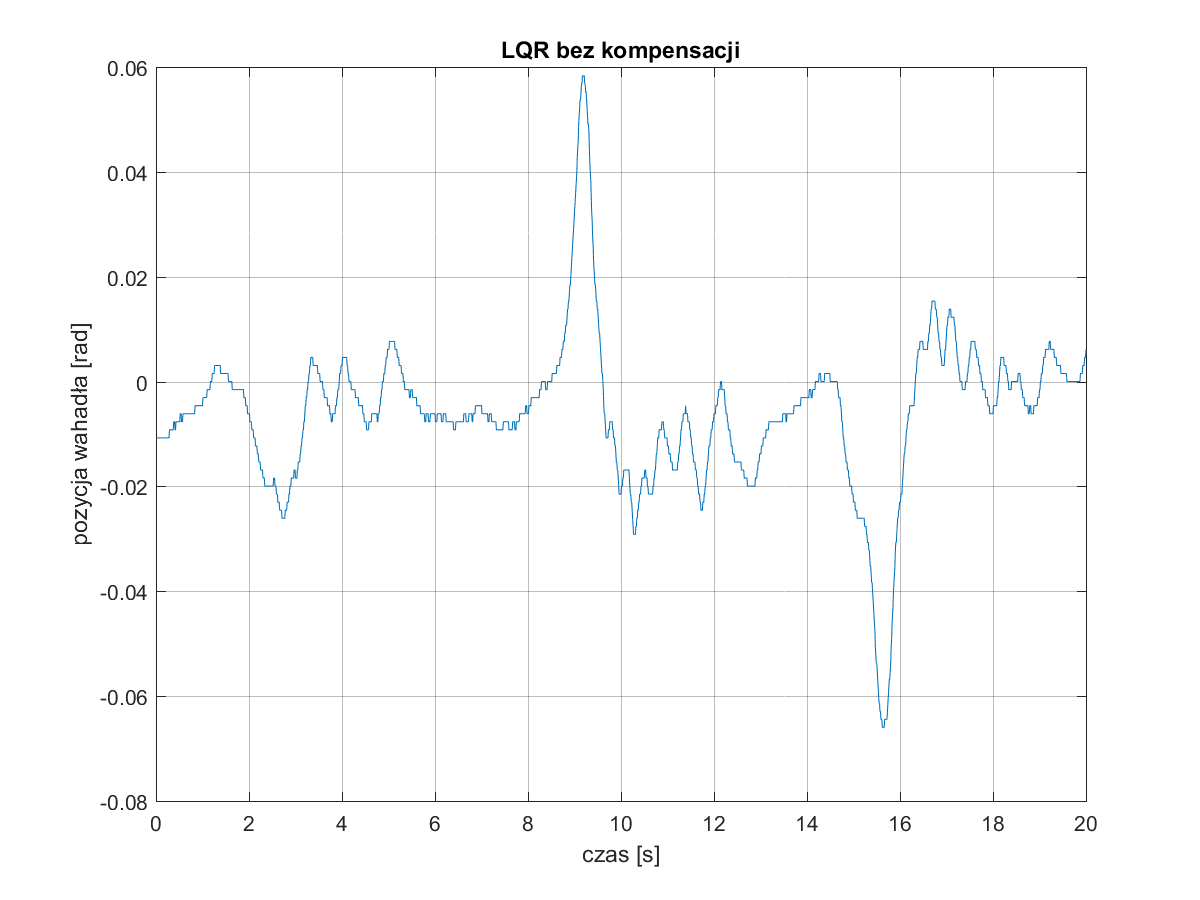
\includegraphics[width=3in]{obrazy/pendulum/LQR_bezk_poz_wah.png}}
	~~
	\subfloat{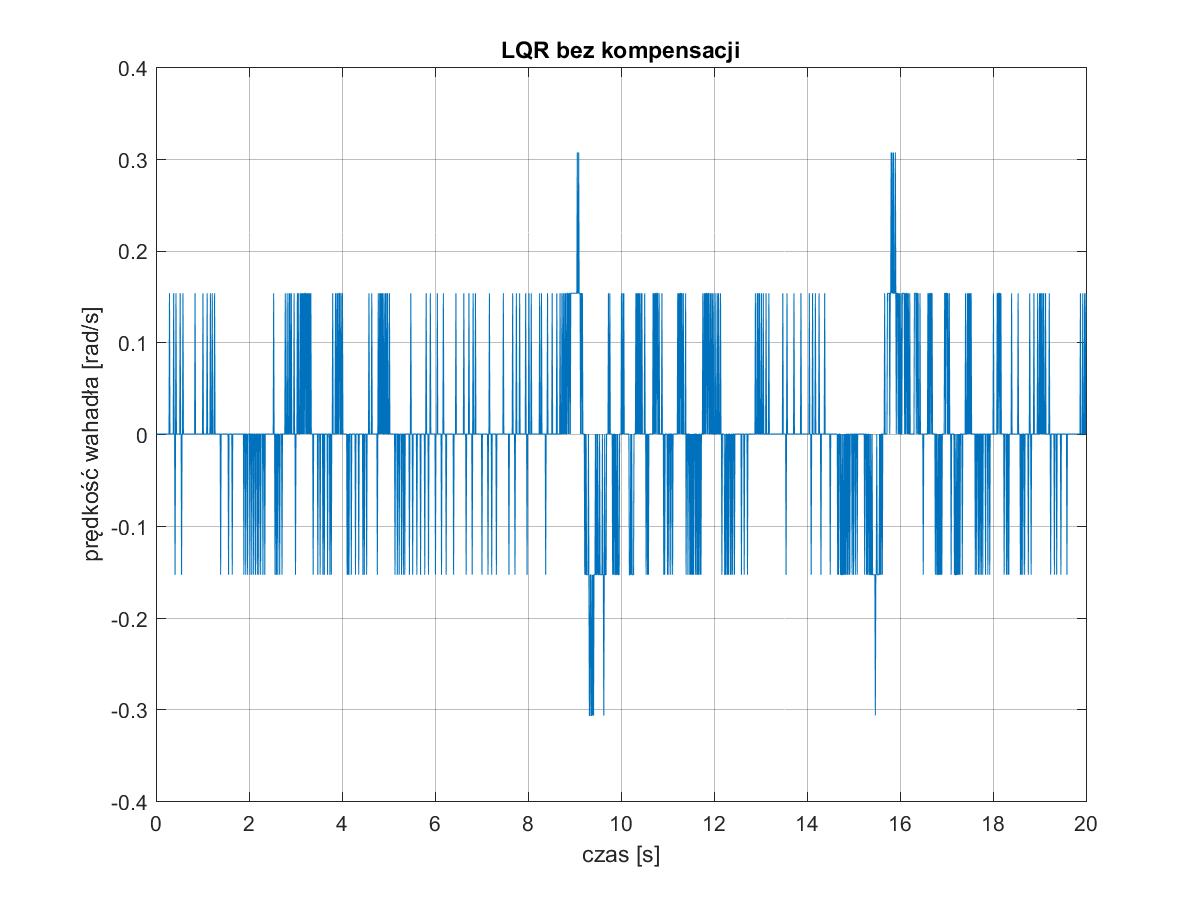
\includegraphics[width=3in]{obrazy/pendulum/LQR_bezk_pred_wah.png}}
	
	\subfloat{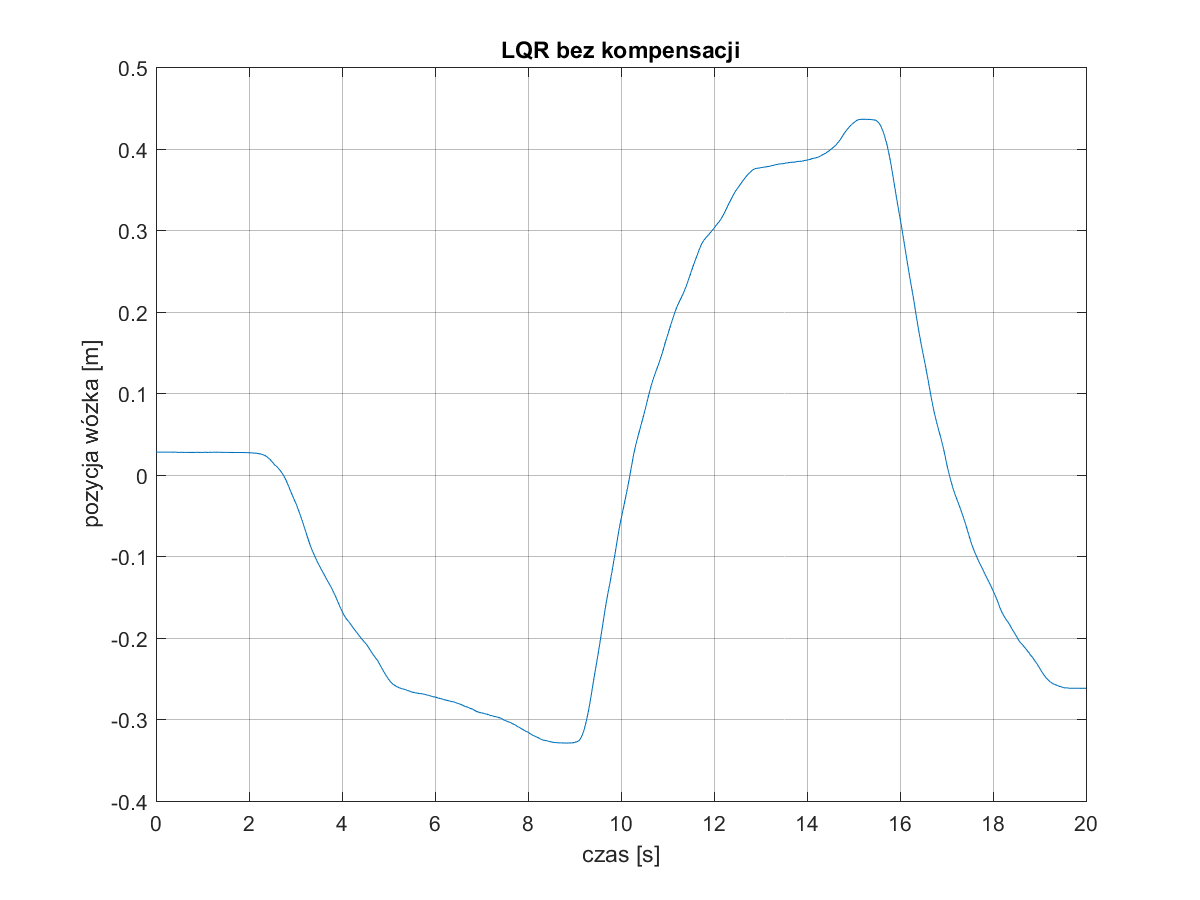
\includegraphics[width=3in]{obrazy/pendulum/LQR_bezk_poz_woz.png}}
	~~
	\subfloat{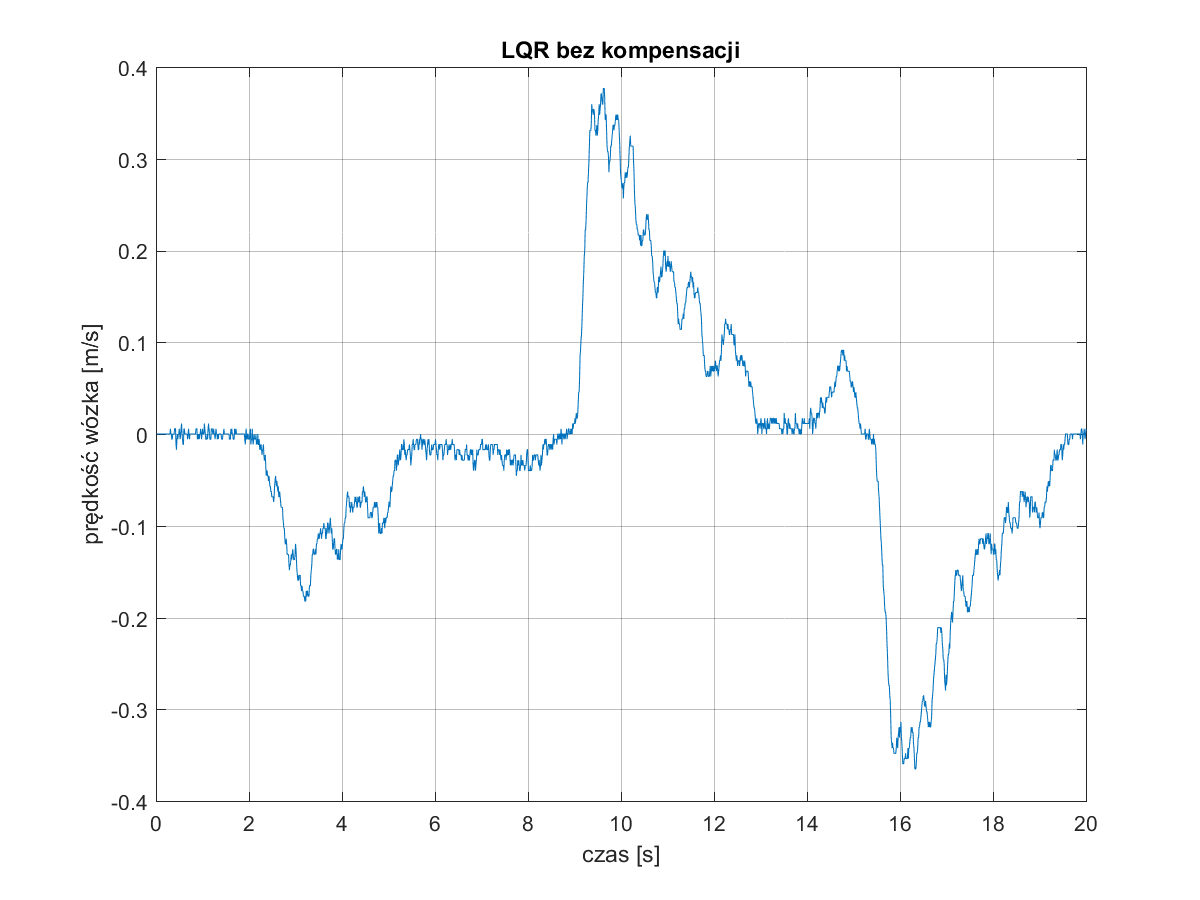
\includegraphics[width=3in]{obrazy/pendulum/LQR_bezk_pred_woz.png}}
	
	\subfloat{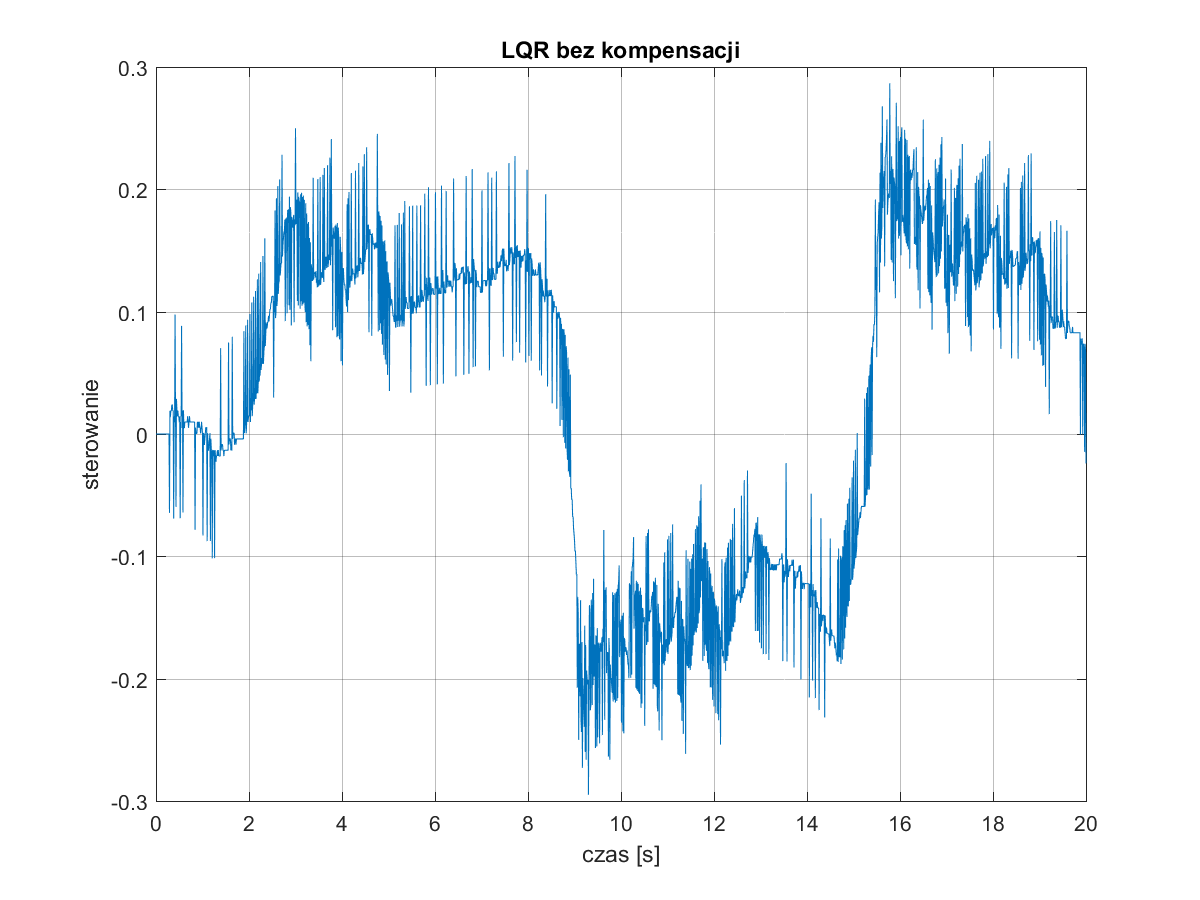
\includegraphics[width=3in]{obrazy/pendulum/LQR_bezk_ster.png}}
%	~~
%	\subfloat{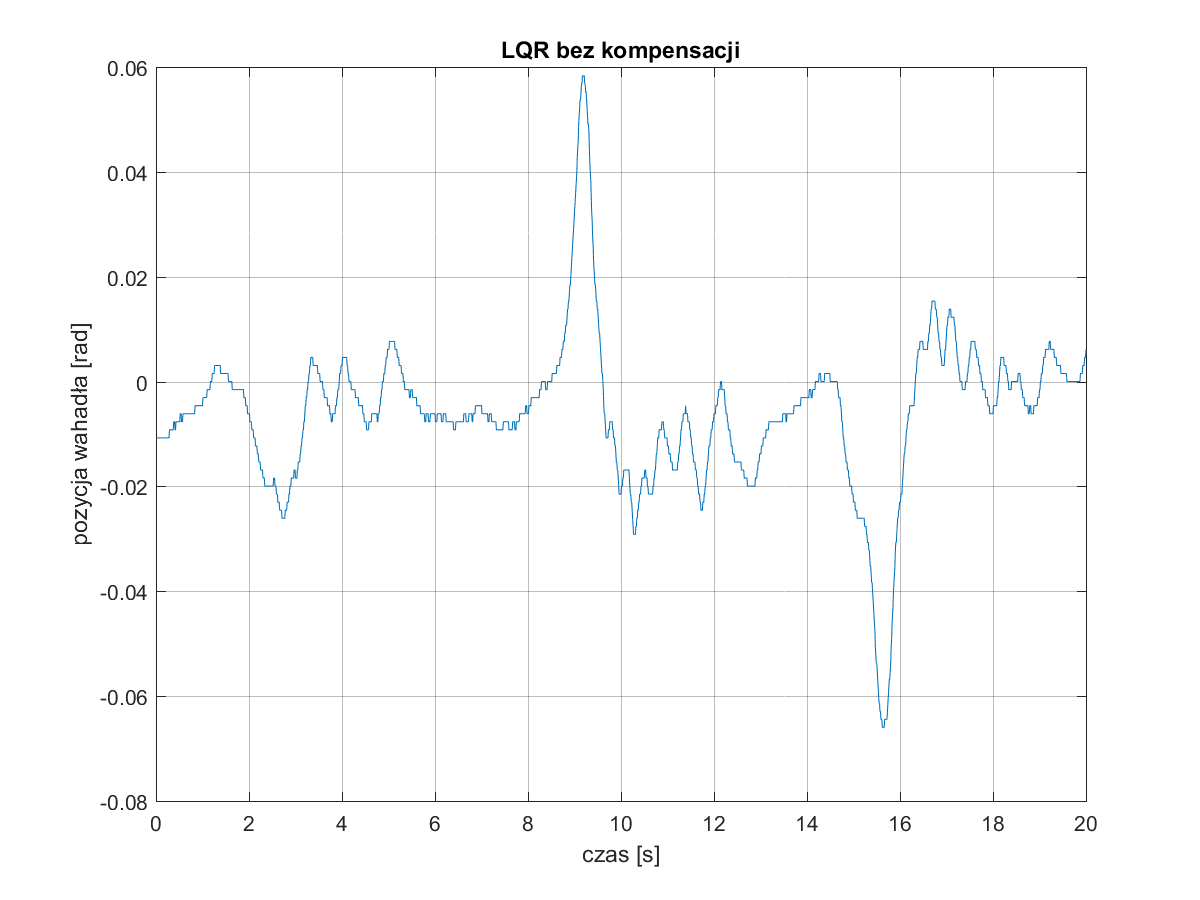
\includegraphics[width=2.8in]{obrazy/pendulum/LQR_bezk_poz_wah.png}}
	\caption{Zadanie stabilizacji obiektu w niestabilnym punkcie równowagi przy użyciu regulatora LQR bez kompensacji tarcia statycznego.}
\label{fig:LQRbezKom}
\end{figure}

Zauważono wpływ tarcia statycznego objawiający się oscylacjami wokół zadanego położenia wózka na szynie.
\subsection{Tarcie statyczne}
Modelowanie tarcia statycznego nie jest prostym zadaniem. Zaobserwowano, że napięcie podawane na silnik potrzebne do pokonania siły tarcia wózka o szynę nie jest stałe, zależy od położenia wózka. Aby zredukować niekorzystny wpływ tarcia na działanie systemu postanowiono wykorzystać następujące podejście. Sterowanie \ref{eq:u} wyliczone przez regulator zostanie zwiększone (w sensie wartości bezwzględnej) o stałą wartość kompensującą siłę tarcia $u_{F_T}=0.11$, która wyznaczona została eksperymentalnie:
\begin{equation}
\label{eq:Kompen}
u(t) = -(Kx(t)+u_{F_T}\cdot sgn(Kx(t))
\end{equation}
\begin{figure}[H]
	\centering
	\subfloat{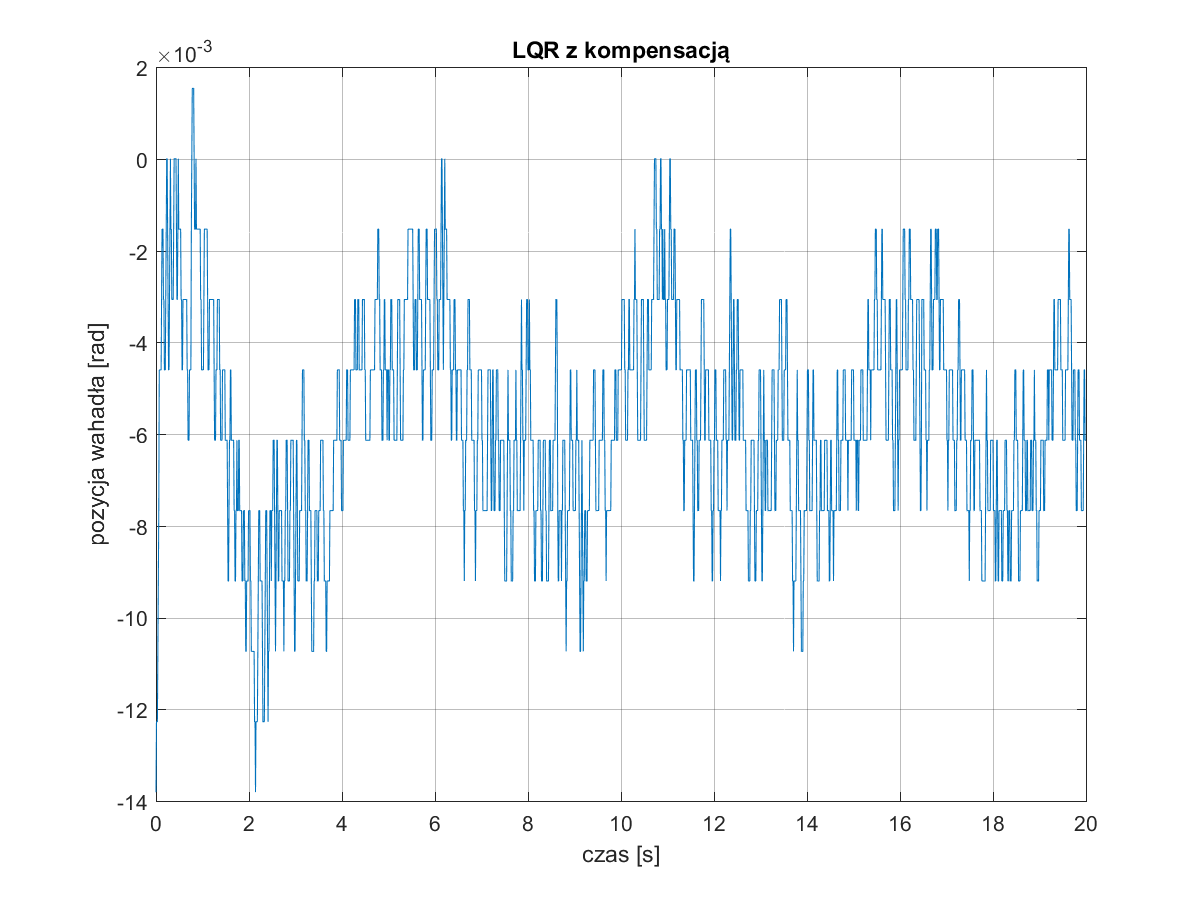
\includegraphics[width=3in]{obrazy/pendulum/LQR_zk_poz_wah.png}}
	~~
	\subfloat{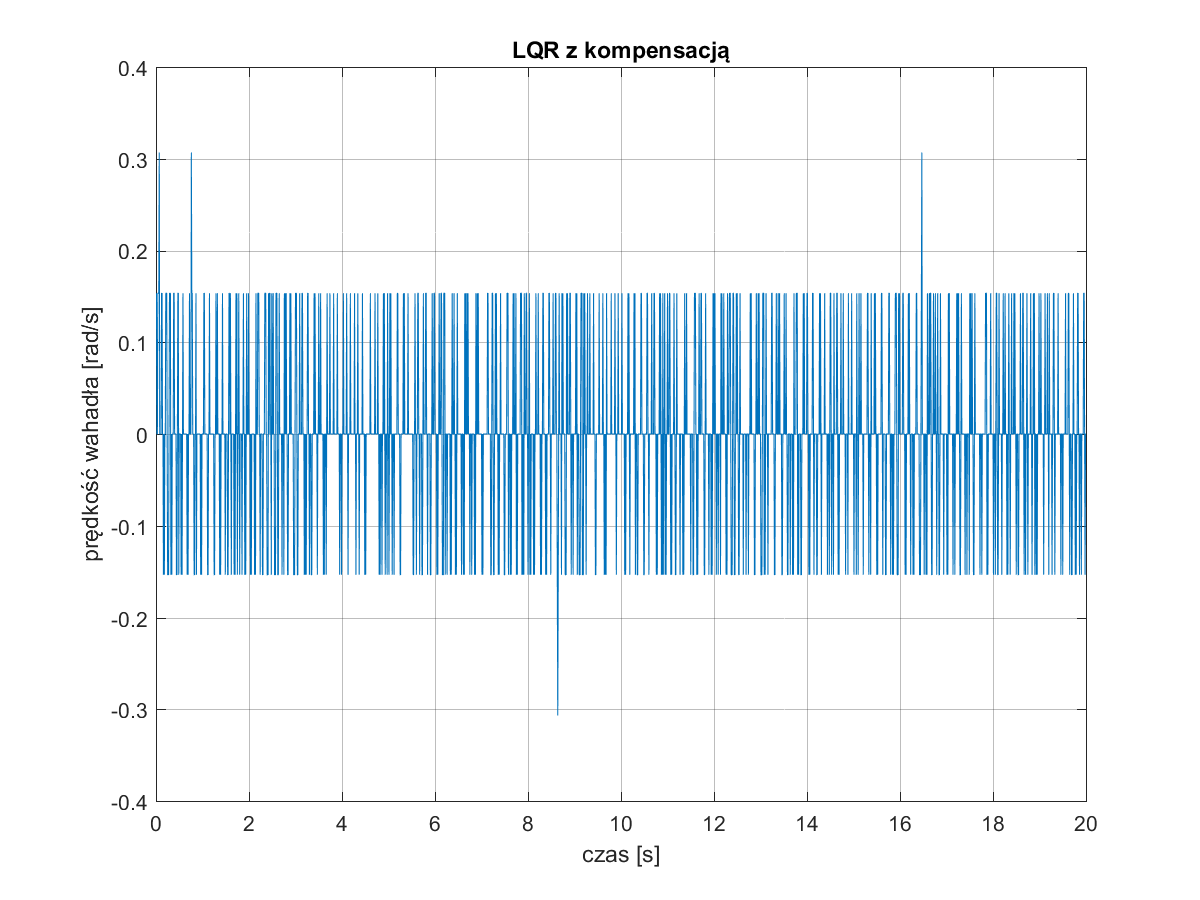
\includegraphics[width=3in]{obrazy/pendulum/LQR_zk_pred_wah.png}}
	
	\subfloat{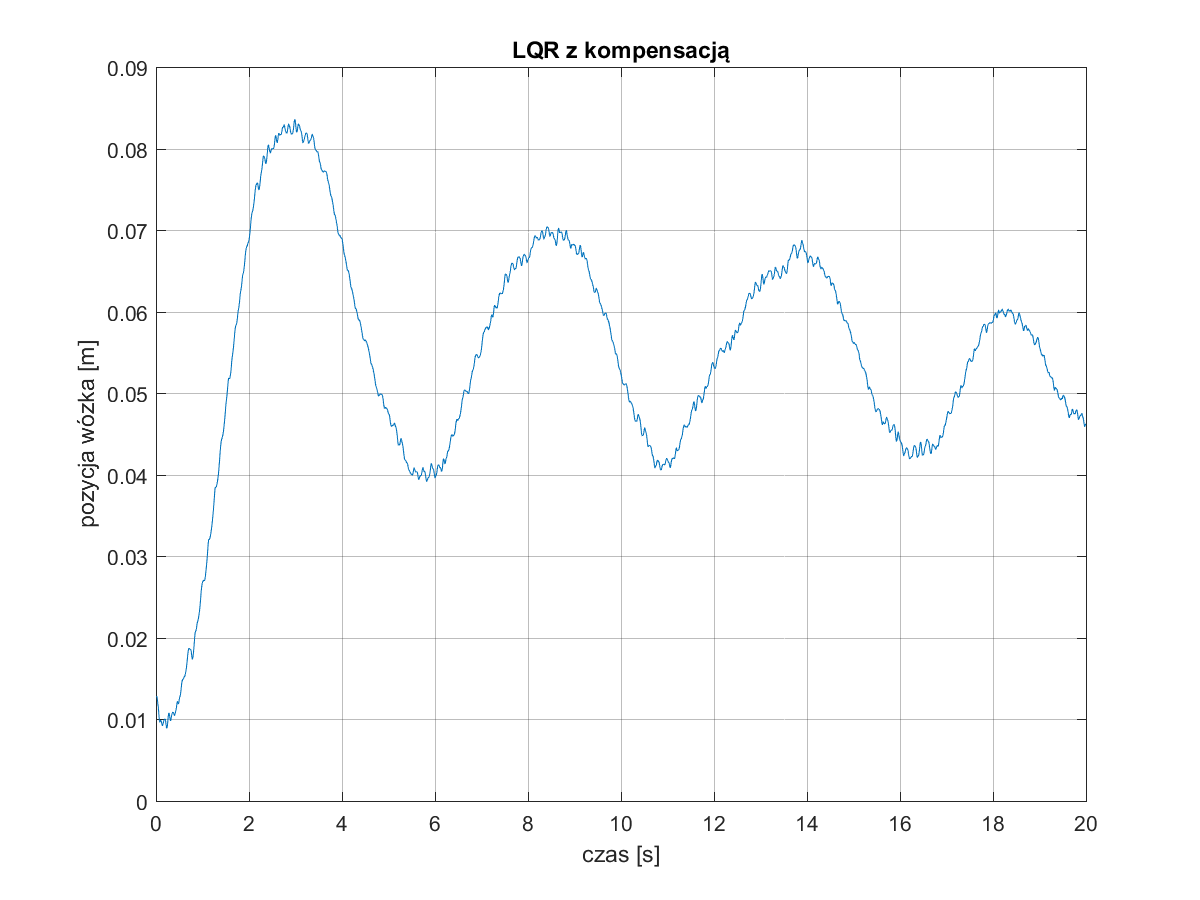
\includegraphics[width=3in]{obrazy/pendulum/LQR_zk_poz_woz.png}}
	~~
	\subfloat{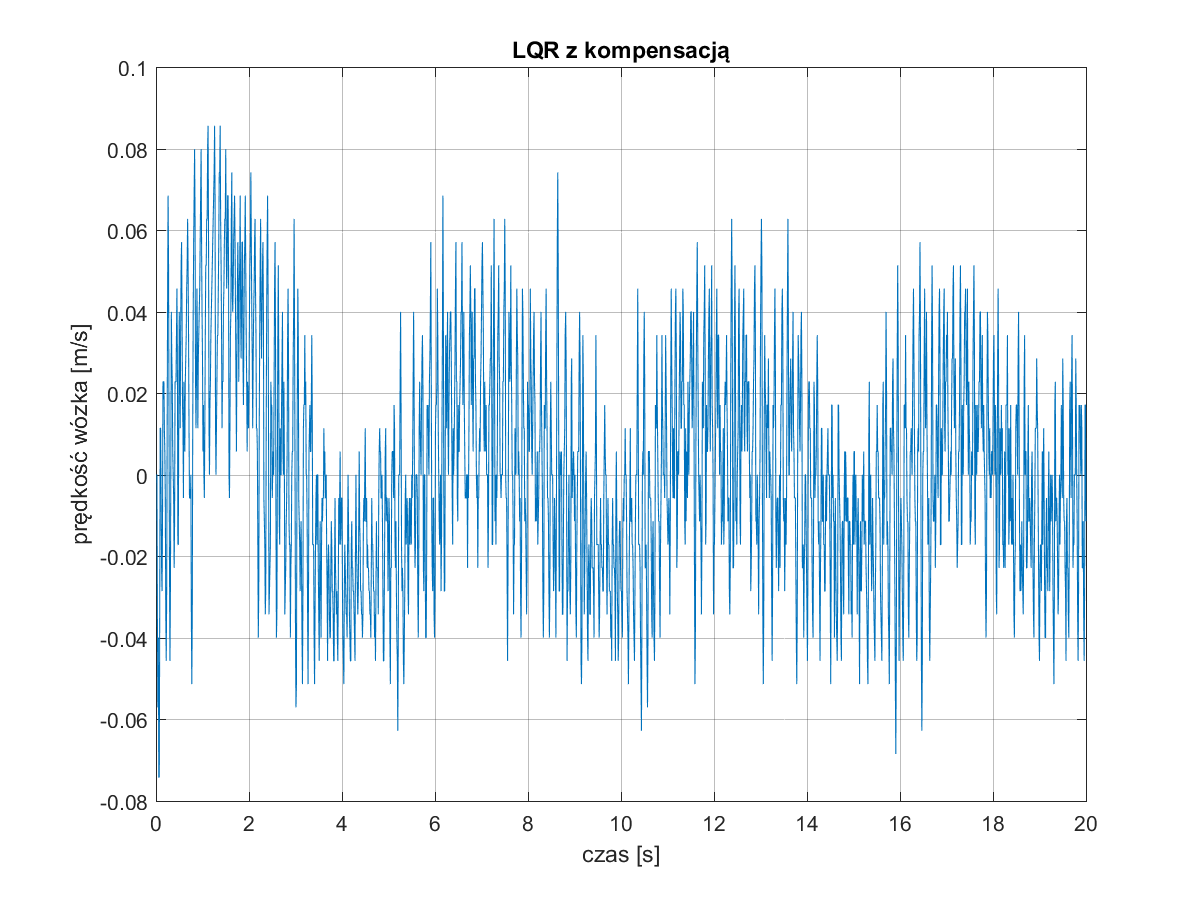
\includegraphics[width=3in]{obrazy/pendulum/LQR_zk_pred_woz.png}}
	
	\subfloat{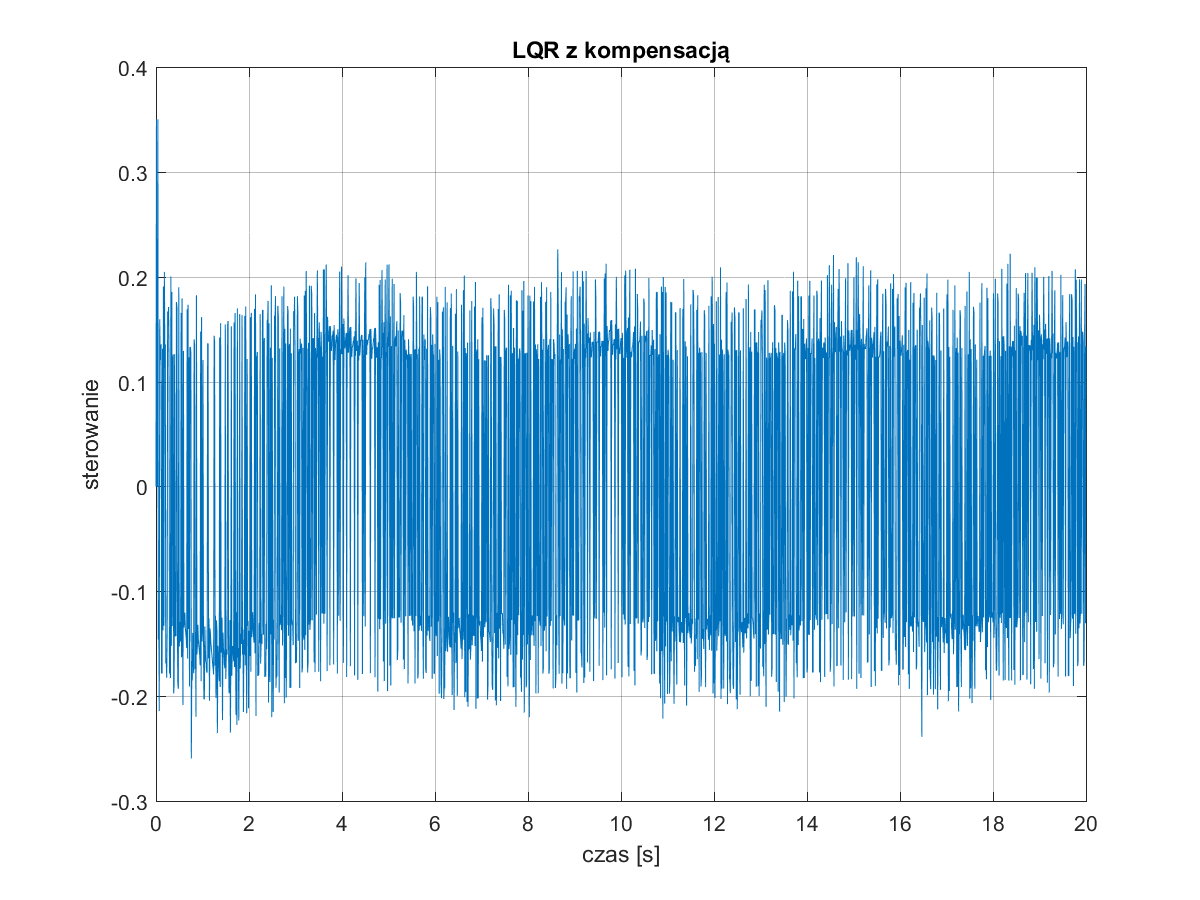
\includegraphics[width=3in]{obrazy/pendulum/LQR_zk_ster.png}}
%	~~
%	\subfloat{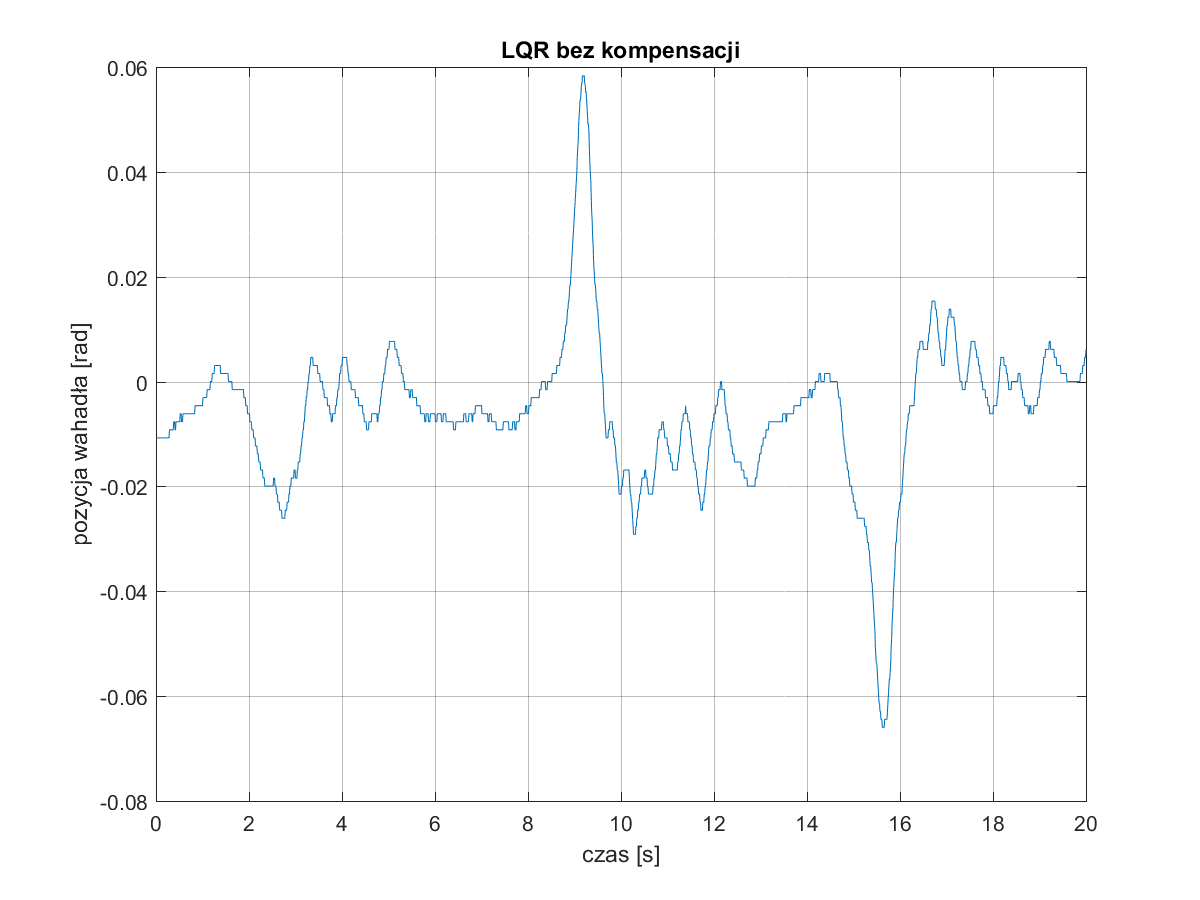
\includegraphics[width=2.8in]{obrazy/pendulum/LQR_bezk_poz_wah.png}}
	\caption{Zadanie stabilizacji obiektu w niestabilnym punkcie równowagi przy użyciu regulatora LQR z kompensacją tarcia statycznego.}
\label{fig:LQRkom}
\end{figure}
Problem oscylacji wózka został w znaczącym stopniu zażegnany. Amplituda wychyleń wózka zmalała blisko dziesięciokrotnie co ukazane zostało na rysunkach \ref{fig:LQRbezKom} oraz \ref{fig:LQRkom}. Zastosowanie regulatora opisanego równaniem \ref{eq:Kompen}  wprowadziło nieciągłości funkcji sterującej w punktach:
 \begin{equation}
\left\lbrace x: Kx(t)=0\right\rbrace 
\end{equation}
Nieciągłości te objawiały się widocznymi drganiami wózka o wysokiej częstotliwości.
% wykres drgań
